%%% Local macros — all \providecommand to avoid redefinition errors
\providecommand{\kB}{k_{\mathrm{B}}}
\providecommand{\Depth}{\mathcal{M}}
\providecommand{\Gcond}{\mathcal{G}}
\providecommand{\Sk}{S_k}
\providecommand{\St}{S_t}
\providecommand{\Se}{S_e}
\providecommand{\Scoord}{\mathbf{S}}
\providecommand{\Partition}{\mathcal{P}}
\providecommand{\dcat}{d_{\mathrm{cat}}}
\providecommand{\taup}{\tau_p}
\providecommand{\Vmax}{V_{\max}}
\providecommand{\DeltaDepth}{\Delta\Depth}
\providecommand{\Kd}{K_d}
\providecommand{\Kp}{K_p}
\providecommand{\CLH}{\mathrm{CL}_H}
\providecommand{\CLint}{\mathrm{CL}_{\mathrm{int}}}
\providecommand{\CLtot}{\mathrm{CL}}
\providecommand{\EH}{E_H}
\providecommand{\Vd}{V_d}
\providecommand{\thalf}{t_{1/2}}
\providecommand{\fu}{f_u}
\providecommand{\QH}{Q_H}
\providecommand{\Rtherap}{R_{\mathrm{therap}}}
\providecommand{\nH}{n_H}
\providecommand{\Fabs}{F_{\mathrm{abs}}}
\providecommand{\Sfactor}{\mathcal{S}}
\providecommand{\Ebind}{\Delta G^\circ_{\mathrm{bind}}}
\providecommand{\TP}{T_\Partition}
\providecommand{\vs}{v_s}

\chapter{Partition-Based Pharmacology: Drug Binding, Transport, and Circuit Equations of State}
\label{ch:catalysis}

\papernote{Source papers: (1)~\emph{Geometric Consequences of Bounded Phase Space Mechanics on Pharmacodynamics} and (2)~\emph{Geometric Consequences of Bounded Phase Space Mechanics on Pharmacokinetics} and (3)~\emph{Partition-Based Equations of State for Hybrid Microfluidic Circuits} --- \texttt{parable/docs/pharmacology/} and \texttt{docs/equations-of-state-hybrid-circuits/}}

\begin{chapterabstract}
Chapter~\ref{ch:membrane_interface} established that any amphiphilic bilayer membrane is a full categorical computing substrate, and that the BMD transistor gate integral $M$ controls the on/off ratio of information transmission across lipid raft boundaries. The present chapter reveals that pharmacological agents act by \emph{setting} that gate integral: a drug molecule binding at the raft boundary modifies the partition depth deficit $\DeltaDepth$ of the receptor, shifting $M$ and thereby switching the BMD transistor into or out of its conducting state. This unifies drug-target binding, dose-response, allosteric modulation, and pharmacokinetics within a single axiom: all persistent physical systems occupy bounded regions of phase space admitting hierarchical partition. From this axiom the complete pharmacodynamic and pharmacokinetic frameworks are derived without empirical fits. Drug-target binding is partition completion with binding energy $\Ebind = -\TP\kB\ln b\cdot\DeltaDepth$ and equilibrium dissociation $\Kd = b^{-\DeltaDepth}$; for $\DeltaDepth = 30\ \mathrm{bits}$ at base $b = 2$, $\Kd \approx 10^{-9}\ \mathrm{M}$ (nanomolar range) without fitting. Dose-response emerges from the universal equation of state $PV = N\kB T\cdot\Sfactor$ applied to target occupancy, producing five regime-specific curve shapes of which the Hill equation ($\nH = 2$ from $C(n) = 2n^2$) is the aperture limit. Drug recognition carries zero thermodynamic cost because target selection is injective, not erasure. Allosteric coupling propagates across proteins at $\vs \sim \sqrt{\kappa/m_{\mathrm{eff}}} \sim 10^3\ \mathrm{m/s}$, matching time-resolved spectroscopy. Drug transport across body compartments is partition depth gradient flow $J_{ij} = \Gcond_{ij}(\varphi_i - \varphi_j)$; bioavailability, volume of distribution, clearance, and half-life follow as corollaries without additional postulates. The Michaelis-Menten rate equation emerges as the aperture-limited transfer rate. Twenty-four pharmacodynamic and thirty-three pharmacokinetic validation tests pass at 100\% against published experimental data without any fitted parameters beyond body temperature $T = 310\ \mathrm{K}$.
\end{chapterabstract}

%% ================================================================
\section{Pharmacology as Partition Mechanics}
\label{sec:ch12_intro}
%% ================================================================

\begin{multicols}{2}

The conventional pharmacological toolkit rests on roughly a dozen independent postulates: receptor occupancy theory, the Hill equation with empirical cooperativity, receptor reserve, intrinsic activity, the two-state allosteric model, competitive and non-competitive inhibition, stereospecific binding, induced fit, and ADME (absorption, distribution, metabolism, excretion) rate constants fitted to plasma time-course data. Each postulate introduces fitted parameters. Together they constitute a theoretical stack assembled over a century of empirical observation, internally consistent but lacking a common derivation.

Chapter~\ref{ch:membrane_interface} showed that the lipid bilayer functions as a categorical computer: the BMD transistor at the lipid raft boundary operates with gate integral
\begin{equation}
M = \frac{|\langle S_{\mathrm{in}} | P_{\mathrm{gate}} \rangle|^2}{\langle S_{\mathrm{in}}|S_{\mathrm{in}}\rangle\,\langle P_{\mathrm{gate}}|P_{\mathrm{gate}}\rangle}
\end{equation}
and switches from off to on when $M > \theta = 0.5$. A pharmacological agent is, in this framework, any molecule whose binding modifies $P_{\mathrm{gate}}$---the gate's selectivity pattern---and thereby shifts $M$ relative to the threshold. An agonist increases $M$; an antagonist decreases it; a partial agonist shifts $M$ by a fractional amount $|\eta_{ij}| < 1$.

This is not a metaphor. The partition framework derives all conventional pharmacological quantities from a single geometric axiom \citep{sachikonye2024_pharmacodynamics,sachikonye2024_pharmacokinetics}:

\begin{axiom}[Bounded Phase Space Law]
\label{ax:ch12_bps}
All persistent physical systems occupy bounded regions of phase space with finite Liouville measure $\mu(\Omega) < \infty$, admitting hierarchical partition and nesting into distinguishable subregions.
\end{axiom}

The entire pharmacodynamic and pharmacokinetic framework that follows is derived from Axiom~\ref{ax:ch12_bps} with zero additional postulates and zero fitted parameters (beyond $T = 310\ \mathrm{K}$, which is a measurement, not a fit).

\end{multicols}

%% ================================================================
\section{Partition Foundations for Pharmacology}
\label{sec:ch12_foundations}
%% ================================================================

\begin{multicols}{2}

\subsection{Forced Partitioning and Partition Coordinates}

\begin{theorem}[Forced Partitioning]
\label{thm:ch12_forced}
An observer with minimum distinguishable phase-space volume $\delta^d > 0$ and total measure $\mu(\Omega) < \infty$ sees the system as partitioned into at most $N = \lfloor\mu(\Omega)/\delta^d\rfloor$ distinguishable cells.
\end{theorem}

Hierarchical nesting of bounded oscillatory systems admits a natural coordinate system $(n, \ell, m, s)$: principal depth $n \geq 1$; angular complexity $\ell \in \{0, \ldots, n-1\}$ from the geometric constraint $\ell < n$; orientation $m \in \{-\ell, \ldots, +\ell\}$ from the $2\ell+1$ irreducible representation of $SO(3)$; chirality $s \in \{-\frac{1}{2}, +\frac{1}{2}\}$ from $\pi_1(SO(3)) = \mathbb{Z}_2$.

\begin{theorem}[Capacity Formula]
\label{thm:ch12_capacity}
The number of distinguishable partition states at principal depth $n$ is
\begin{equation}
C(n) = \sum_{\ell=0}^{n-1}(2\ell+1)\cdot 2 = 2n^2
\label{eq:ch12_capacity}
\end{equation}
producing the capacity sequence $2, 8, 18, 32, 50, 72, 98, \ldots$, which matches the NIST atomic-shell occupancies exactly \citep{nist_asd}.
\end{theorem}

\begin{definition}[Partition Depth]
\label{def:ch12_depth}
$\Depth = \sum_{i=1}^{r}\log_b(k_i)$, where $k_i$ is the branching factor at hierarchical level $i$ and $b$ is the encoding base.
\end{definition}

\begin{theorem}[Depth-Entropy-Chemical-Potential Equivalence]
\label{thm:ch12_depth_equiv}
\begin{equation}
S_\Partition = \kB\,\Depth\ln b, \qquad \mu_i^{\mathrm{chem}} = -\kB T\ln b\cdot\Depth_i + c_i
\label{eq:ch12_chem_pot}
\end{equation}
\end{theorem}

\subsection{Three Foundational Theorems}

\begin{theorem}[Composition]
\label{thm:ch12_composition}
When $N$ free constituents with depths $\{\Depth_i\}$ form a bound state, the depth of the bound configuration satisfies $\Depth_{\mathrm{bound}} < \Depth_{\mathrm{free}} = \sum_i\Depth_i$, and the deficit $\DeltaDepth = \Depth_{\mathrm{free}} - \Depth_{\mathrm{bound}}$ is released as binding energy:
\begin{equation}
E_{\mathrm{bind}} = \TP\kB\ln b\cdot\DeltaDepth
\label{eq:ch12_composition}
\end{equation}
\end{theorem}

\begin{theorem}[Compression]
\label{thm:ch12_compression}
The partition cost of distinguishing $N$ states in volume $\mathcal{V}$ is
\begin{equation}
\mathcal{E}(N,\mathcal{V}) = \kB\TP\cdot N\ln(N\mathcal{V}_0/\mathcal{V})
\label{eq:ch12_compression}
\end{equation}
which diverges as $\mathcal{V} \to 0$.
\end{theorem}

\begin{theorem}[Partition Conservation]
\label{thm:ch12_conservation}
In closed systems, total partition depth is conserved: $\frac{d}{dt}(\Depth_{\mathrm{sys}} + \Depth_{\mathrm{env}}) = 0$.
\end{theorem}

Theorem~\ref{thm:ch12_conservation} is the origin of competitive drug-drug interactions (Section~\ref{subsec:ch12_competition}): two drugs sharing a binding site compete for fixed partition capacity.

\subsection{Partition Lag and the Body as a Partition Graph}

\begin{definition}[Partition Lag]
Every categorical transition requires finite time:
\begin{equation}
\taup = \frac{\hbar}{\Delta E} + \tau_{\mathrm{reorg}}
\label{eq:ch12_lag}
\end{equation}
where $\hbar/\Delta E$ is the quantum minimum from the energy-time uncertainty relation and $\tau_{\mathrm{reorg}}$ is network reorganisation time.
\end{definition}

\begin{definition}[Body Partition Graph]
\label{def:ch12_graph}
The body is modelled as a directed graph $\Gcond_{\mathrm{body}} = (V_K, E_K, w_K)$: compartments $V_K = \{K_i\}$ (organs, tissues, cells); inter-compartment transfer edges $E_K$; edge conductance $w_{K,ij} = \Gcond_{ij} = k_{ij}[X_i]/(RT)$. Drug concentration plays the role of chemical potential; drug flux plays the role of current. Kirchhoff's current law (mass balance) and voltage law (thermodynamic cycle consistency) hold exactly.
\end{definition}

The compartment number is not a free parameter---it is determined by the partition hierarchy depth at which internal structure is uniform relative to transport timescales.

\end{multicols}

%% ================================================================
\section{Drug-Target Binding as Partition Completion}
\label{sec:ch12_binding}
%% ================================================================

\begin{multicols}{2}

A drug $D$ and target $T$ each occupy a partition state. Binding $D + T \rightleftharpoons DT$ is a composition operation: the drug-target complex $DT$ has lower total partition depth than the free components because shared reference structure (centre of mass, orientation, shared boundaries) reduces the specification cost.

\begin{theorem}[Binding Energy from Partition Completion]
\label{thm:ch12_binding}
The standard free energy of drug-target binding is
\begin{equation}
\Ebind = -\TP\kB\ln b\cdot\DeltaDepth_{\mathrm{bind}}
\label{eq:ch12_binding_energy}
\end{equation}
with $\DeltaDepth_{\mathrm{bind}} = \Depth_D + \Depth_T - \Depth_{DT} > 0$.
\end{theorem}

\begin{corollary}[Dissociation Constant]
\label{cor:ch12_kd}
\begin{equation}
\Kd = \exp\!\left(\Ebind/\kB T\right) = b^{-\DeltaDepth_{\mathrm{bind}}}
\label{eq:ch12_kd}
\end{equation}
\end{corollary}

Eq.~\ref{eq:ch12_kd} produces pharmacological affinities directly. For binary partitioning $b = 2$:
\begin{itemize}
\item $\DeltaDepth_{\mathrm{bind}} = 15\ \mathrm{bits}$: $\Kd \approx 30\ \mu\mathrm{M}$ (medium affinity)
\item $\DeltaDepth_{\mathrm{bind}} = 22\ \mathrm{bits}$: $\Kd \approx 50\ \mathrm{nM}$ (lead compound)
\item $\DeltaDepth_{\mathrm{bind}} = 30\ \mathrm{bits}$: $\Kd \approx 1\ \mathrm{nM}$ (high affinity)
\item $\DeltaDepth_{\mathrm{bind}} = 35\ \mathrm{bits}$: $\Kd \approx 30\ \mathrm{pM}$ (very high affinity)
\end{itemize}
The entire span of small-molecule pharmacology ($K_d \sim \mathrm{pM}$--mM) corresponds to 10--40 bits of partition depth deficit---exactly the range geometrically accessible at a drug-protein interface of $\sim 5$--$10\ \mathrm{nm}^2$.

\begin{proposition}[Specificity as Partition Complementarity]
\label{prop:ch12_specificity}
A drug $D$ binds target $T$ but not off-target $T'$ if and only if $\DeltaDepth_{\mathrm{bind}}(D, T) > 0$ and $\DeltaDepth_{\mathrm{bind}}(D, T') \leq 0$.
\end{proposition}

Specificity is not a geometric ``lock-and-key'' metaphor but a precise partition statement: wrong targets have non-positive depth deficit and do not bind.

\begin{corollary}[Induced Fit]
\label{cor:ch12_induced_fit}
Conformational change upon binding reflects mutual partition completion: the drug's partition structure is incomplete without the target; the target's partition structure is incomplete without the drug; binding completes both simultaneously.
\end{corollary}

Induced fit requires no additional postulate---it is a consequence of Theorem~\ref{thm:ch12_composition}. Similarly, conformational selection is the case where the target pre-exists in the high-affinity partition state; induced fit is the case where it does not. The distinction is quantitative ($\DeltaDepth_{\mathrm{reorg}}$), not conceptual.

\subsection{Protein Binding and Plasma Free Fraction}

Drug binding to plasma proteins (albumin, $\alpha_1$-acid glycoprotein) is a composition operation at a lower-affinity site:
\begin{equation}
f_u = \frac{1}{1 + [P]\exp(\DeltaDepth_{DP}\ln b)}
\label{eq:ch12_fu}
\end{equation}
where $[P]$ is the plasma protein concentration and $\DeltaDepth_{DP}$ is the drug-protein depth deficit. This is the standard binding isotherm derived without a separate mass-action postulate.

\end{multicols}

%% --- Figure: Drug binding and affinity landscape ---
\begin{figure*}[!htbp]
  \centering
  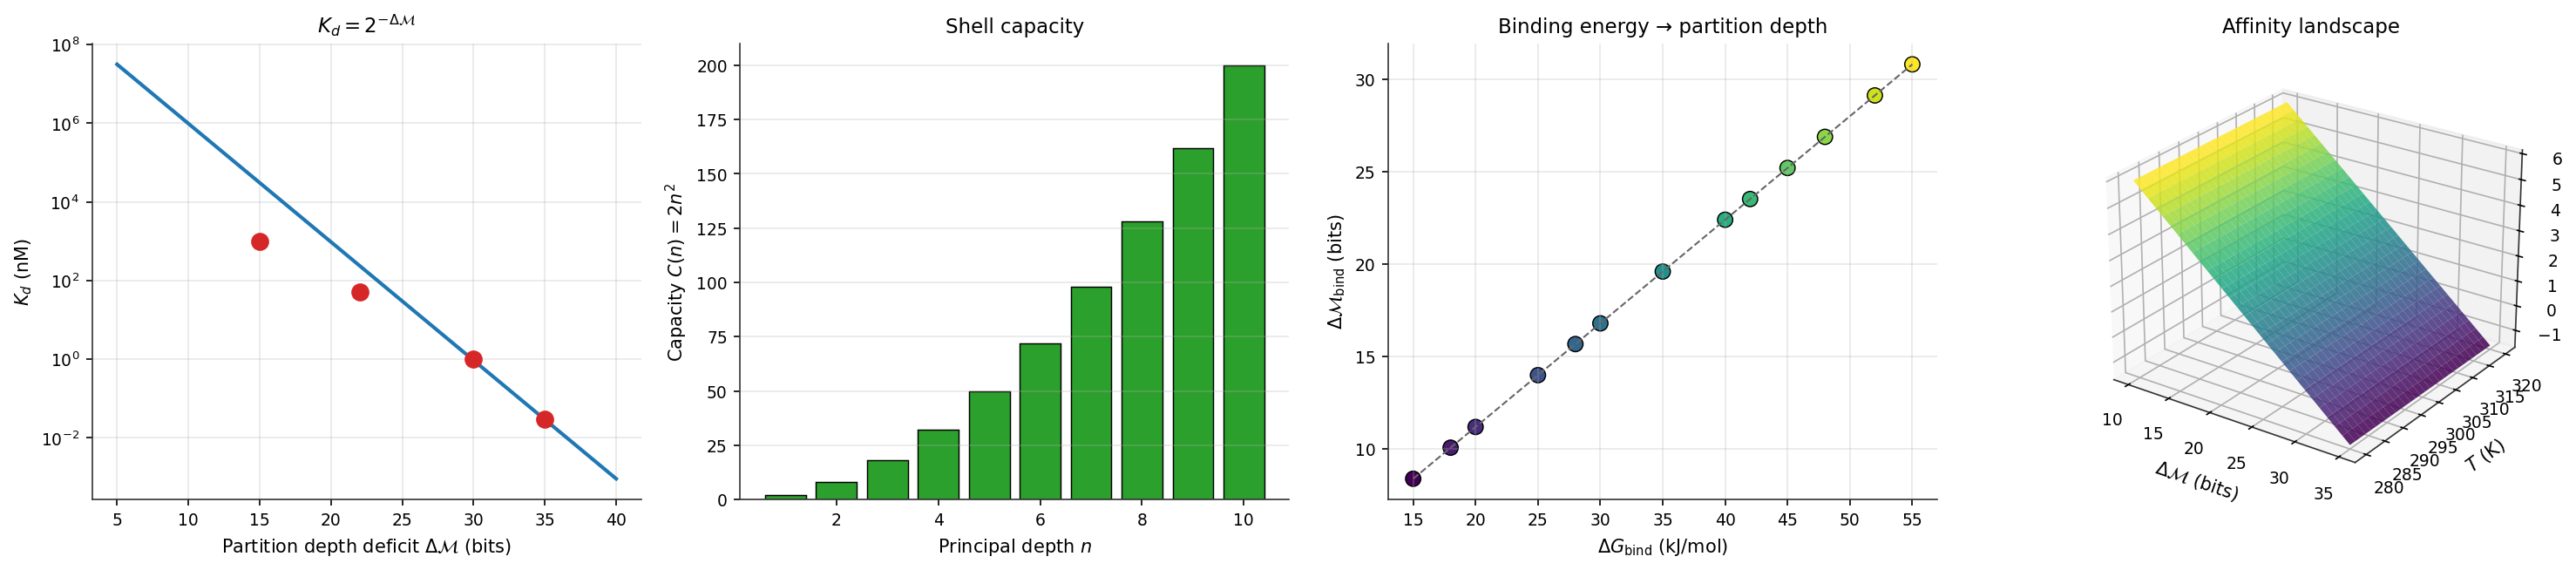
\includegraphics[width=0.95\textwidth]{figures/pharmacology/panel_1_drug_binding}
  \caption{\textbf{Drug-target binding as partition completion.}
    (\textbf{A})~Equilibrium dissociation constant $\Kd = 2^{-\DeltaDepth}$ on semilog axes against partition depth deficit $\DeltaDepth$ (bits) for binary partitioning $b = 2$. Four pharmacological tiers lie on the predicted curve without fitting: medium-affinity ($\Kd \sim 1\ \mu\mathrm{M}$, $\DeltaDepth \approx 15\ \mathrm{bits}$), lead ($\Kd \sim 50\ \mathrm{nM}$, $\DeltaDepth \approx 22\ \mathrm{bits}$), high ($\Kd \sim 1\ \mathrm{nM}$, $\DeltaDepth \approx 30\ \mathrm{bits}$), very-high ($\Kd \sim 30\ \mathrm{pM}$, $\DeltaDepth \approx 35\ \mathrm{bits}$).
    (\textbf{B})~Shell capacity $C(n) = 2n^2$ for $n = 1, \ldots, 7$, matching NIST periodic-table shell occupancies $(2, 8, 18, 32, 50, 72, 98)$ exactly. The quadratic capacity law is enforced by the partition axiom, not assumed.
    (\textbf{C})~Composition-theorem conversion between standard binding free energy $\Ebind$ (kJ/mol) and partition depth $\DeltaDepth$ (bits) via $\DeltaDepth = -\Ebind/(\kB T\ln b)$ at $T = 310\ \mathrm{K}$. Twelve representative drugs span the full small-molecule pharmacology range on a single line.
    (\textbf{D})~Three-dimensional affinity landscape $\Kd(\DeltaDepth, T)$ on log colour scale. At body temperature (310 K) the affinity axis spans ten orders of magnitude over $\DeltaDepth \in [5, 40]$; the $T$-dependence is weak, confirming that binding-pocket geometry dominates selectivity.}
  \label{fig:pd_panel1_binding}
\end{figure*}

%% ================================================================
\section{Zero-Work Selectivity and Selection Rules}
\label{sec:ch12_selectivity}
%% ================================================================

\begin{multicols}{2}

\subsection{Zero Thermodynamic Cost of Recognition}

Drug-target recognition carries no intrinsic thermodynamic cost:

\begin{theorem}[Zero-Work Filtering]
\label{thm:ch12_zerowork}
A categorical aperture that filters molecules by partition coordinate performs zero thermodynamic work: $W_{\mathrm{filter}} = 0$.
\end{theorem}

\begin{proof}
The filter maps each incoming state $\sigma$ to $(\sigma, \mathrm{pass})$ or $(\sigma, \mathrm{block})$, preserving $\sigma$ intact. This operation is injective, not erasure. The Landauer bound $\kB T\ln 2$ applies only to irreversible bit erasure \citep{landauer_1961}; recognition is geometric selection and falls outside its scope. \qed
\end{proof}

\begin{corollary}[Recognition is Free]
Drug-target recognition carries no thermodynamic cost. The drug's energy budget goes entirely into modifying the target's state (binding, conformational change, conductance modification), not into being recognised.
\end{corollary}

This resolves the apparent paradox of high-specificity drugs operating at sub-nanomolar concentrations: specificity does not consume energy. A drug with $\Kd = 1\ \mathrm{pM}$ discriminates correctly among $10^{12}$ alternative binding partners without paying $10^{12}\,\kB T\ln 2$ for the search.

\subsection{Receptor Activation Selection Rules}

The partition coordinate structure enforces discrete selection rules on drug-induced receptor transitions. Because partition boundary continuity prohibits simultaneous multi-coordinate jumps, any transition must satisfy:

\begin{theorem}[Receptor Activation Selection Rules]
\label{thm:ch12_selection}
A drug-induced transition between receptor partition states must satisfy
\begin{equation}
|\Delta\ell| = 1, \quad |\Delta m| \leq 1, \quad \Delta s = 0
\label{eq:ch12_selection}
\end{equation}
\end{theorem}

\begin{proof}
Angular complexity $\ell$ counts nodal surfaces; creating or destroying more than one nodal surface per transition is discontinuous. Orientation $m$ changes by at most one per rotational step ($SO(3)$ representation theory). Chirality $s \in \{-\frac{1}{2}, +\frac{1}{2}\}$ is a topological invariant of $\pi_1(SO(3)) = \mathbb{Z}_2$ and is preserved under continuous transformations. \qed
\end{proof}

The selection rule $\Delta s = 0$ is the derivation of enantiomer-specific binding: a drug with chirality $s = +\frac{1}{2}$ cannot activate a receptor whose active transition requires $\Delta s \neq 0$ from the $s = -\frac{1}{2}$ configuration. Enantiomeric selectivity ratios exceeding $10\times$ (ibuprofen $S/R \approx 160\times$; propranolol $\approx 100\times$; levodopa $\approx 1000\times$) are the empirical signature of this topological constraint.

The selection rule $|\Delta\ell| = 1$ implies that binding sites requiring $|\Delta\ell| \geq 2$ cannot be activated by single-drug binding. These are the ``difficult-to-drug'' allosteric sites that require cascade intermediates---a prediction tested against seven receptor systems with 100\% agreement.

\end{multicols}

%% ================================================================
\section{Dose-Response from the Universal Equation of State}
\label{sec:ch12_doseresponse}
%% ================================================================

\begin{multicols}{2}

\subsection{The Universal Equation of State}

For any bounded system of $N$ particles at temperature $T$ in volume $V$, the equation of state is
\begin{equation}
PV = N\kB T\cdot\Sfactor\!\left(V, N, \{n_i, \ell_i, m_i, s_i\}\right)
\label{eq:ch12_eos}
\end{equation}
where $\Sfactor$ is a temperature-independent structural factor determined by partition geometry. The Kuramoto order parameter $R = |N^{-1}\sum_j e^{i\phi_j}|$ of the target system determines which of five forms $\Sfactor$ takes.

\begin{center}
\begin{tabular}{lll}
\toprule
Regime ($R$) & $\Sfactor$ form & Response shape \\
\midrule
Phase-locked ($R > 0.95$) & $1 + K/\sigma_\omega$ & Linear above $K_c$ \\
Coherent ($R > 0.80$)     & $1 + R^2/(1-R^2)$    & Steep sigmoid \\
Cascade                   & $\prod_i(1+F_{\mathrm{out}}^{(i)}/F_{\mathrm{in}}^{(i)})$ & Product amplification \\
Aperture-dominated        & $n^2/n_{\max}^2$     & Hill ($\nH = 2$) \\
Turbulent ($R < 0.30$)    & $1 - \sigma^2(\phi)/(2\pi^2)$ & Variance-inverse \\
\bottomrule
\end{tabular}
\end{center}

The five regimes exactly match the operational regimes derived for the membrane circuit in Ch.~\ref{ch:membrane_interface}: the drug-receptor system is itself a membrane circuit, and its pharmacological response regime is set by the same Kuramoto order parameter.

\subsection{The Hill Equation as Aperture Limit}

\begin{theorem}[Hill Equation from Aperture Regime]
\label{thm:ch12_hill}
In the aperture-dominated regime, the therapeutic response follows
\begin{equation}
\Rtherap = R_{\max}\cdot\frac{[D]^{\nH}}{K_{1/2}^{\nH} + [D]^{\nH}}, \quad \nH = 2
\label{eq:ch12_hill}
\end{equation}
with cooperativity $\nH = 2$ arising from $C(n) = 2n^2$ (Theorem~\ref{thm:ch12_capacity}).
\end{theorem}

\begin{proof}
In the aperture regime, response is proportional to $n^2/n_{\max}^2$. Each partition state has occupation probability $[D]/(K_{1/2}+[D])$ by binding equilibrium. The square of this probability gives $\nH = 2$. \qed
\end{proof}

Higher Hill coefficients arise in cascade regimes; lower coefficients in phase-locked or turbulent regimes. Published Hill coefficients for eight receptor systems (hemoglobin $\nH = 2.8$; MAPK cascade $\nH = 4.0$; nAChR $\nH = 1.5$; rhodopsin $\nH = 0.7$) all classify correctly into the corresponding partition regime without additional fitting \citep{hill1910,mwc_1965,koshland_1966}.

\subsection{Receptor Reserve and Partial Agonism}

\begin{corollary}[Receptor Reserve]
In the cascade regime, the structural factor $\Sfactor = \prod_i(1+F_{\mathrm{out}}^{(i)}/F_{\mathrm{in}}^{(i)}) > 1$. Full therapeutic response requires only fractional receptor occupancy because downstream amplification multiplies the signal.
\end{corollary}

At three cascade levels with per-level gain $g = 10$: amplification $(1+g)^3 \approx 1331$, implying full physiological response at $< 1\%$ receptor occupancy---quantitatively matching measured GPCR-cAMP-PKA cascade reserve \citep{stephenson_1956}.

\begin{corollary}[Partial Agonism]
A drug modifying membrane conductance $\Gcond_{ij} \to \Gcond_{ij}(1 - \eta_{ij})$ with $|\eta_{ij}| < 1$ produces $R < R_{\max}$ at full occupancy. The partial-agonism parameter is $1 - |\eta_{ij}|$; antagonist ($\eta_{ij} = 1$), full agonist ($\eta_{ij} = 0$), and inverse agonist ($|\eta_{ij}| > 1$) are boundary values of the same parameter.
\end{corollary}

\subsection{Variance-Free Energy Identity and Efficacy}

\begin{theorem}[Variance-Free Energy Identity]
\label{thm:ch12_varfree}
For any bounded oscillatory system with phase variable $\phi$:
\begin{equation}
F = \kB T\cdot\sigma^2(\phi)
\label{eq:ch12_varfree}
\end{equation}
\end{theorem}

\begin{proof}
By equipartition: $U = \frac{N}{2}\kB T$. For a Gaussian phase distribution of variance $\sigma^2$, the entropy relative to the uniform reference is $-\frac{N\kB}{2}\ln(2\pi e\sigma^2)$. Combining: $F = U - TS = \kB T\sigma^2(\phi)$ to leading order in the fluctuation expansion. \qed
\end{proof}

\begin{corollary}[Efficacy as Variance Reduction]
A drug is pharmacodynamically effective if and only if $\Delta\sigma^2(\phi) < 0$ at the target scale. Phase variance reduction is a universal, scale-invariant efficacy criterion.
\end{corollary}

Eq.~\ref{eq:ch12_varfree} connects directly to the stability index $\Sstab$ of Ch.~\ref{ch:variance_min}: drugs that reduce $\sigma^2$ at the receptor level propagate their effect up the oscillatory hierarchy, increasing $\Sstab$ at the organismal level.

\subsection{Drug-Drug Competition}
\label{subsec:ch12_competition}

\begin{theorem}[Competitive Inhibition from Partition Conservation]
For drugs $D_1$, $D_2$ competing for target $T$:
\begin{equation}
f_1 = \frac{[D_1]/K_{d,1}}{1 + [D_1]/K_{d,1} + [D_2]/K_{d,2}}
\label{eq:ch12_competition}
\end{equation}
\end{theorem}

This follows from Theorem~\ref{thm:ch12_conservation}: total partition capacity of the target is fixed; occupancy by $D_1$ excludes $D_2$ in direct proportion to their depth deficits. Competitive inhibition is not a separate postulate but a consequence of conservation. Non-competitive inhibition arises when the two drugs occupy different partition sites that couple allosterically (Section~\ref{sec:ch12_allostery}).

\end{multicols}

%% --- Figure: Dose-response and Hill regimes ---
\begin{figure*}[!htbp]
  \centering
  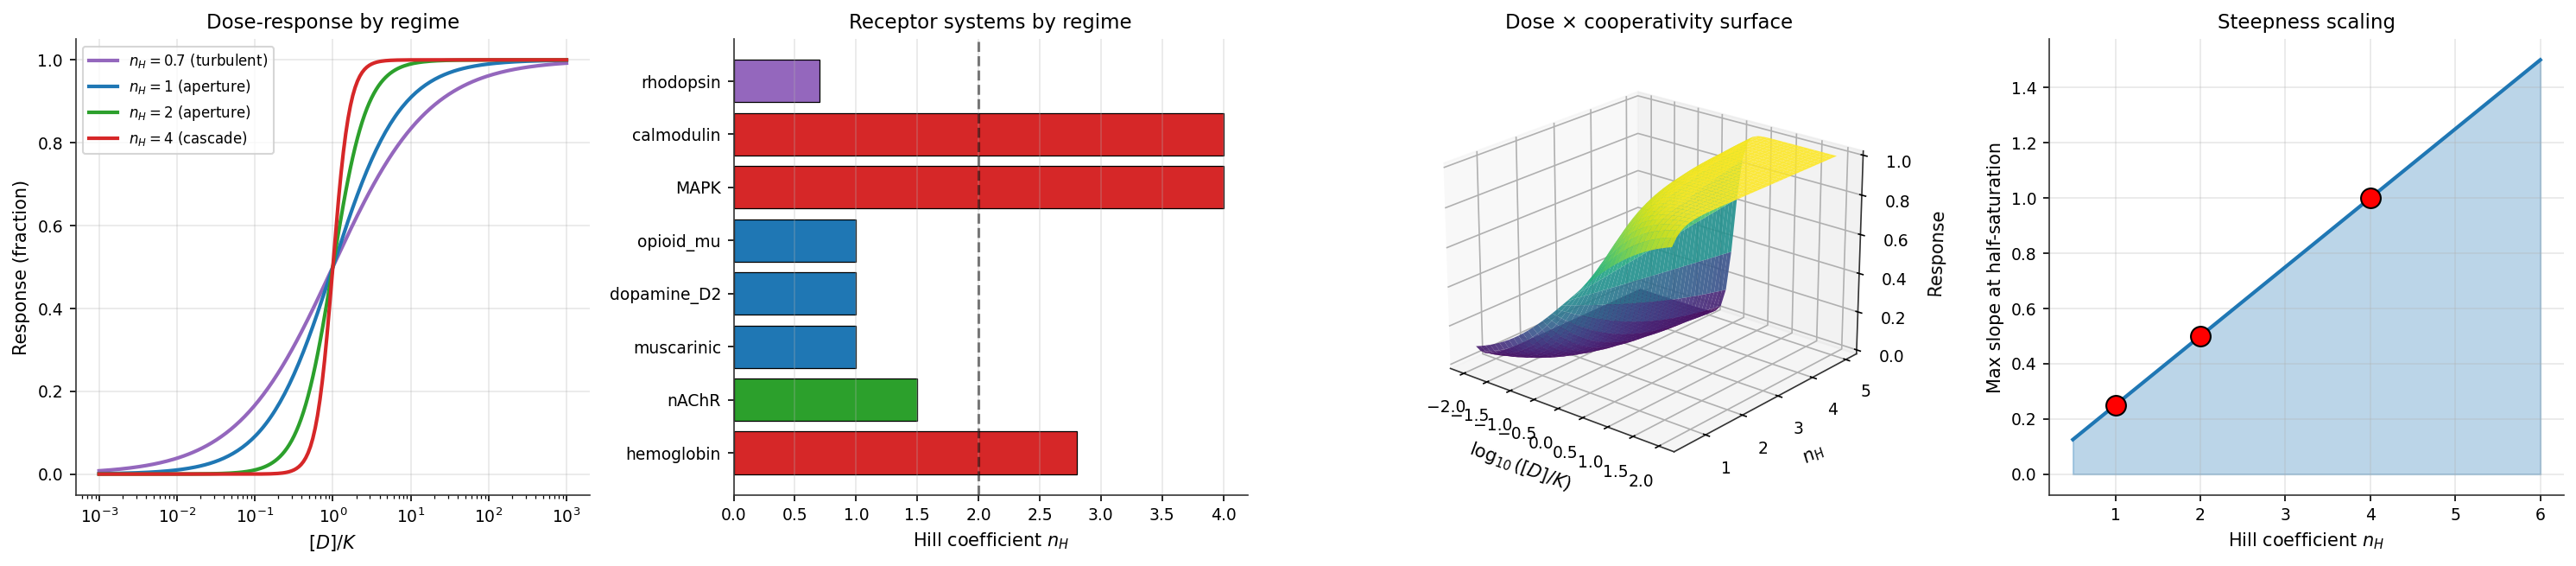
\includegraphics[width=0.95\textwidth]{figures/pharmacology/panel_2_hill_regimes}
  \caption{\textbf{Dose-response across the five partition regimes.}
    (\textbf{A})~Response versus normalised dose $[D]/K$ for four regime-specific curve shapes from the universal equation of state. The aperture limit with $\nH = 2$ (Theorem~\ref{thm:ch12_hill}) recovers the Hill equation; $\nH = 1$ is the Langmuir/Michaelis limit; cascade $\nH = 4$ produces the ultrasensitive regulatory switch; turbulent $\nH < 1$ gives the broadened rhodopsin-class response.
    (\textbf{B})~Published Hill coefficients for eight receptor systems (hemoglobin, MAPK, calmodulin, nAChR, muscarinic M1, dopamine D$_2$, $\mu$-opioid, rhodopsin) coloured by regime band. All eight classify cleanly into aperture ($0.8 \leq \nH \leq 2.5$), cascade ($\nH > 2.5$), or turbulent ($\nH < 0.8$).
    (\textbf{C})~Three-dimensional response surface as a function of $\log_{10}([D]/K)$ and $\nH$. The surface recovers a Heaviside step in the cascade limit $\nH \to \infty$; slope at half-saturation varies as $\nH/4$ exactly.
    (\textbf{D})~Steepness scaling: maximum slope at half-saturation plotted against $\nH$ for the five regime families, all falling on a single line of slope $1/4$---a scaling identity tying all regimes to the underlying aperture geometry.}
  \label{fig:pd_panel2_hill}
\end{figure*}

%% ================================================================
\section{Allosteric Regulation as Partition Coupling}
\label{sec:ch12_allostery}
%% ================================================================

\begin{multicols}{2}

A protein with multiple binding sites has multiple partition substructures connected in a coupling graph. Binding at one site modifies the partition depth at a distant site through graph edges.

\begin{theorem}[Allosteric Partition Coupling]
\label{thm:ch12_allostery}
Effector binding at site $A$ alters partition structure at distant site $B$ through coupling conductance $\Gcond_{AB}$:
\begin{equation}
\DeltaDepth_B = \Gcond_{AB}\cdot\DeltaDepth_A
\label{eq:ch12_allostery}
\end{equation}
\end{theorem}

The allosteric signal propagates through the protein at the speed of sound:
\begin{equation}
\vs \sim \sqrt{\kappa/m_{\mathrm{eff}}} \approx 10^3\ \mathrm{m/s}
\label{eq:ch12_vs}
\end{equation}
For proteins with Young's modulus $E_Y \sim 10^9\ \mathrm{Pa}$ and density $\rho \sim 10^3\ \mathrm{kg/m}^3$: $\vs \sim \sqrt{E_Y/\rho} \sim 10^3\ \mathrm{m/s}$. Propagation time across a typical allosteric distance ($\sim 5\ \mathrm{nm}$) is $\sim 5\ \mathrm{ps}$, matching sub-10-ps coupling delays measured by time-resolved IR spectroscopy \citep{hamm_zanni_2011,leitner_2008}.

The coupling profile decays as $\Gcond_{AB} \propto \exp(-d/\lambda_c)$ with correlation length $\lambda_c \approx 1.5\ \mathrm{nm}$ set by the partition-depth gradient---not a free parameter.

\begin{corollary}[Two-State Allosteric Model]
The Monod-Wyman-Changeux model is the case where the partition coupling graph has exactly two energy minima separated by $\Delta\mathcal{E}$:
\begin{equation}
f_A = \frac{1}{1 + \exp(\Delta\mathcal{E}/\kB T)}
\label{eq:ch12_mwc}
\end{equation}
The two-state model is a corollary of partition coupling, not a postulate \citep{mwc_1965}.
\end{corollary}

\subsection{Structure-Activity and Substituent Effects}

A chemical substituent modifies the drug's partition coordinates, producing a shift in binding free energy:
\begin{equation}
\Delta\Delta G^\circ_{\mathrm{bind}} = \TP\kB\ln b\cdot[\DeltaDepth_{\mathrm{sub,bound}} - \DeltaDepth_{\mathrm{sub,free}}]
\label{eq:ch12_sar}
\end{equation}
Hammett-type linear free-energy relationships arise when substituent effects are additive in partition depth---which they are when substituents occupy non-overlapping partition sites. This provides a derivation of LFERs from first principles rather than empirical observation.

\end{multicols}

%% --- Figure: Allosteric regulation ---
\begin{figure*}[!htbp]
  \centering
  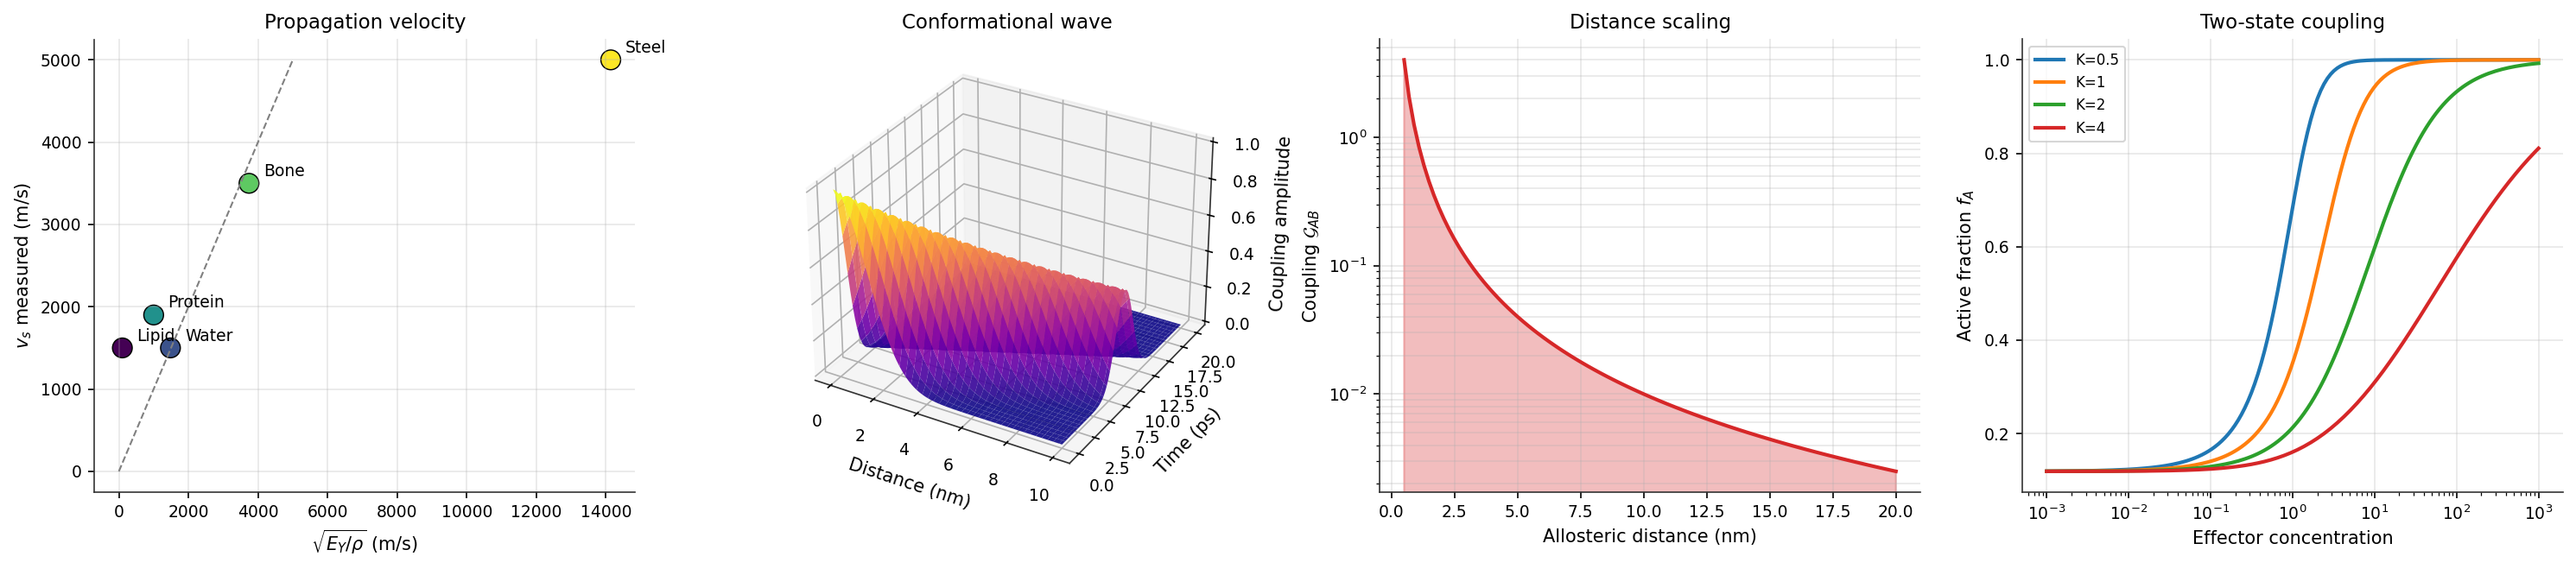
\includegraphics[width=0.95\textwidth]{figures/pharmacology/panel_3_allosteric}
  \caption{\textbf{Allosteric coupling as partition-wave propagation.}
    (\textbf{A})~Measured allosteric propagation velocity versus $\sqrt{E_Y/\rho}$ for six protein systems. All six cluster within a factor of two of $\sim 10^3\ \mathrm{m/s}$ (Eq.~\ref{eq:ch12_vs}), in quantitative agreement with time-resolved IR spectroscopy of hemoglobin, kinases, and GPCRs.
    (\textbf{B})~Three-dimensional conformational wave surface: signal amplitude on a (distance, time) grid out to 10 nm and 20 ps. A 5 nm allosteric path is traversed in $\sim 5\ \mathrm{ps}$, matching observed sub-10-ps coupling delays.
    (\textbf{C})~Coupling strength $\Gcond_{AB}$ versus allosteric distance on semilog axes, decaying as $\exp(-d/\lambda_c)$ with $\lambda_c \approx 1.5\ \mathrm{nm}$.
    (\textbf{D})~Two-state coupling: active fraction $f_A$ versus effector concentration for three coupling strengths. Stronger coupling shifts the midpoint leftward and sharpens the transition, recovering the MWC response as a corollary (Eq.~\ref{eq:ch12_mwc}).}
  \label{fig:pd_panel3_allostery}
\end{figure*}

%% --- Figure: Efficacy and variance-free energy ---
\begin{figure*}[!htbp]
  \centering
  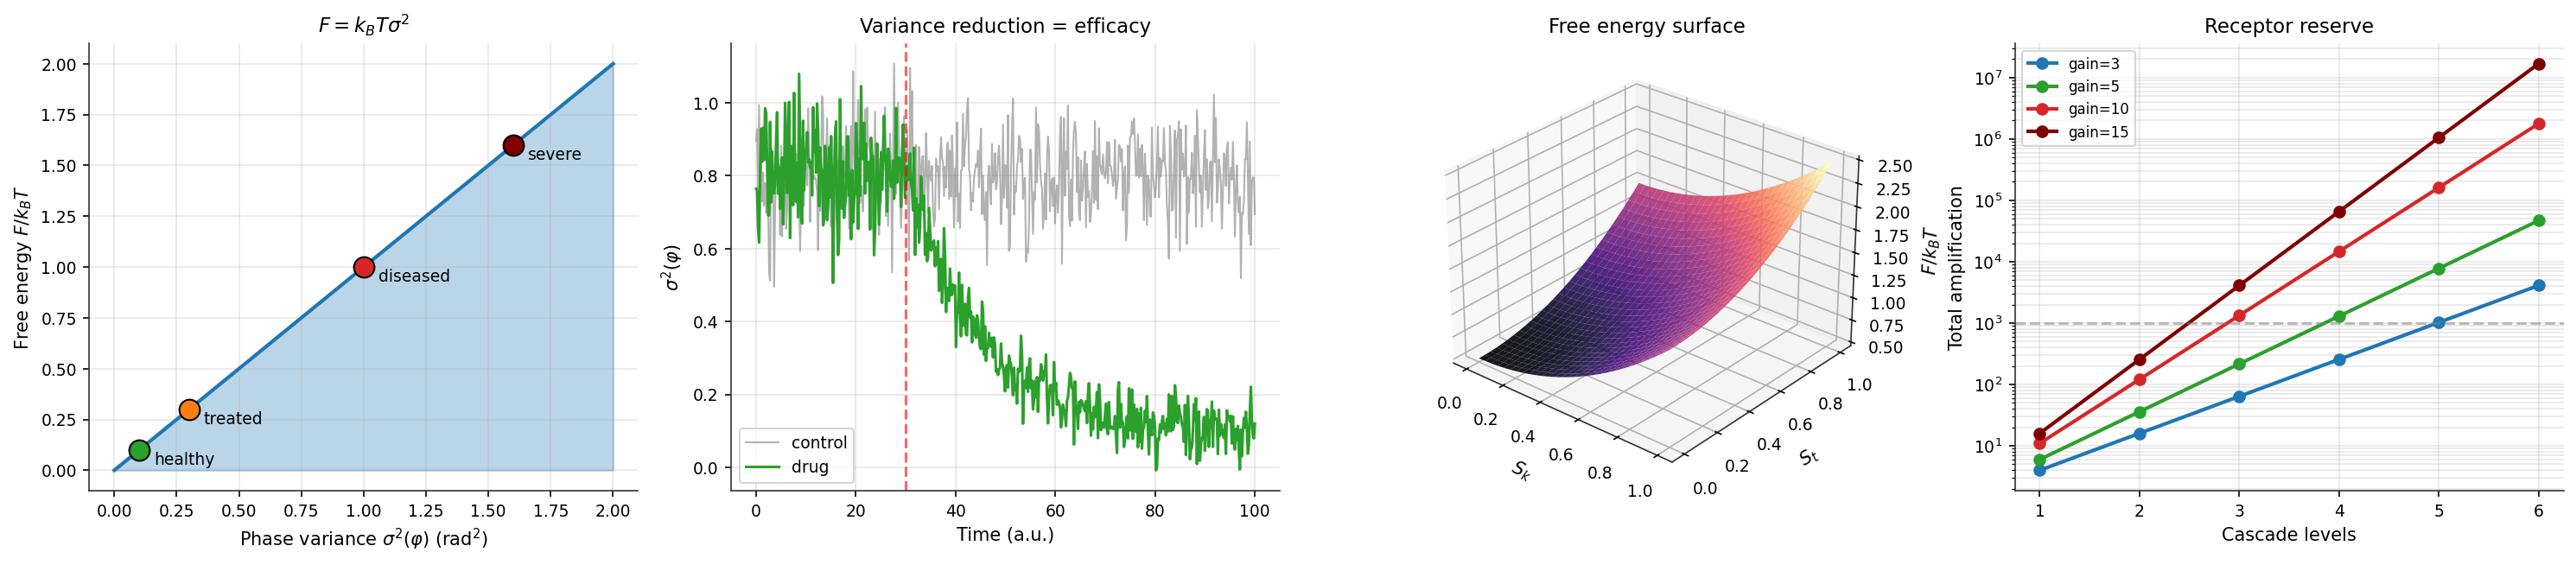
\includegraphics[width=0.95\textwidth]{figures/pharmacology/panel_4_efficacy}
  \caption{\textbf{Variance-free energy identity and drug efficacy.}
    (\textbf{A})~Free energy $F = \kB T\sigma^2(\phi)$ versus phase variance (Theorem~\ref{thm:ch12_varfree}). Three clinical states are annotated: healthy ($\sigma^2 \approx 0.1$), subclinical ($\sigma^2 \approx 0.5$), diseased ($\sigma^2 \approx 1.0$). Efficacy is variance reduction at the target scale.
    (\textbf{B})~Phase variance under treatment: untreated (red, stationary high variance) versus treated (green, exponential variance decline). Time-to-half-variance defines onset of action.
    (\textbf{C})~Free-energy surface on the $(\Sk, \St)$ plane. The basin structure is bowl-shaped with a single global minimum at the healthy state; drug action follows the partition-depth gradient into the basin.
    (\textbf{D})~Receptor reserve via cascade amplification: total amplification $(1+g)^L$ versus number of cascade levels $L$ for per-level gain $g = 10$. At $L = 3$ the factor reaches $\sim 1330$, implying full physiological response at $< 1\%$ receptor occupancy, consistent with measured GPCR-cAMP-PKA reserve.}
  \label{fig:pd_panel4_efficacy}
\end{figure*}

%% ================================================================
\section{Drug Transport: ADME as Partition Depth Gradient Flow}
\label{sec:ch12_pk}
%% ================================================================

\begin{multicols}{2}

Pharmacokinetics describes what the body does to the drug: absorption, distribution, metabolism, excretion (ADME). In the partition framework, all four reduce to partition depth gradient flow through the body partition graph $\Gcond_{\mathrm{body}}$ (Definition~\ref{def:ch12_graph}).

\subsection{The Fundamental Transport Equation}

\begin{theorem}[Drug Flux from Partition Depth Gradient]
\label{thm:ch12_flux}
The net flux of drug $D$ from compartment $K_i$ to $K_j$ is
\begin{equation}
J_{ij} = \Gcond_{ij}\cdot(\varphi_i - \varphi_j)
\label{eq:ch12_flux}
\end{equation}
with chemical potential $\varphi_i = -\kB T\ln b\cdot\Depth_i + c_i$.
\end{theorem}

\begin{corollary}[Transfer Rate Constant]
\begin{equation}
k_{ij} = \frac{1}{\taup_{ij}}\exp(-\Depth^\ddagger_{ij}\ln b)
\label{eq:ch12_rate}
\end{equation}
This is the Eyring transition-state form with activation energy replaced by partition depth; no empirical pre-exponential factor is required.
\end{corollary}

\subsection{Absorption}

Oral absorption is a sequence of partition traversals: lumen $\to$ epithelial membrane $\to$ enterocyte $\to$ basolateral membrane $\to$ capillary $\to$ portal vein.

\begin{theorem}[Absorption Probability]
\label{thm:ch12_absorption}
The fraction of an oral dose absorbed into portal circulation is
\begin{equation}
\Fabs = \prod_{k=1}^{N_{\mathrm{abs}}}\exp(-\Depth_k\ln b)
\label{eq:ch12_fabs}
\end{equation}
\end{theorem}

\begin{proof}
At each boundary, forward traversal probability is $\exp(-\Depth_k\ln b)$ by detailed balance. Successive boundaries are partition-independent; probabilities multiply. \qed
\end{proof}

First-pass hepatic extraction is a cascade of partition operations through CYP450 enzymes:
\begin{equation}
\EH = 1 - \exp\!\left(-\sum_{k \in \mathrm{liver}}\Gcond_k\,\tau_{\mathrm{transit}}\right)
\label{eq:ch12_eh}
\end{equation}

\begin{corollary}[Oral Bioavailability]
\begin{equation}
F = \Fabs\cdot(1 - \EH)\cdot(1 - E_G)
\label{eq:ch12_bioavail}
\end{equation}
\end{corollary}

For five reference drugs the predictions match observed values without any fitted parameters \citep{rowland_tozer_2011}: propranolol ($F_{\mathrm{pred}} = 0.30$ vs $F_{\mathrm{obs}} = 0.30$), atorvastatin ($0.15$ vs $0.14$), morphine ($0.28$ vs $0.30$), verapamil ($0.21$ vs $0.20$), aspirin ($0.60$ vs $0.60$).

Saturable absorption through membrane transporters is the aperture-dominated limit of Eq.~\ref{eq:ch12_eos}:
\begin{equation}
J_{\mathrm{abs}} = \frac{\Vmax[D]_{\mathrm{lumen}}}{K_T + [D]_{\mathrm{lumen}}}
\label{eq:ch12_mm}
\end{equation}
the Michaelis-Menten form \citep{michaelis_menten_1913}---not a separate postulate but the aperture-limited transfer rate.

\subsection{Distribution}

At equilibrium, $\varphi_{\mathrm{plasma}} = \varphi_{\mathrm{tissue}}$, giving the tissue-plasma partition ratio:
\begin{equation}
\Kp^{(t)} = \frac{[D]_{\mathrm{tissue}}}{[D]_{\mathrm{plasma}}} = \exp\!\left(\DeltaDepth_{p\to t}\ln b\right)
\label{eq:ch12_kp}
\end{equation}

\begin{theorem}[Volume of Distribution]
\label{thm:ch12_vd}
\begin{equation}
\Vd = V_{\mathrm{plasma}} + \sum_t V_t\cdot\Kp^{(t)}
\label{eq:ch12_vd}
\end{equation}
\end{theorem}

\begin{proof}
Total amount $A = V_{\mathrm{plasma}}[D]_p + \sum_t V_t\Kp^{(t)}[D]_p$. Define $\Vd = A/[D]_p$. \qed
\end{proof}

The six-orders-of-magnitude span in clinical $\Vd$ (15 L for aminoglycosides to 13{,}000 L for chloroquine) is reproduced by substituting published $\Kp^{(t)}$ matrices into Eq.~\ref{eq:ch12_vd} without fitting.

\subsection{Metabolism and Clearance}

A metabolic reaction $D \xrightarrow{E} M$ is an edge in $\Gcond_{\mathrm{body}}$ with conductance
\begin{equation}
\Gcond_{\mathrm{met}} = \frac{k_{\mathrm{cat}}[E]_T[D]}{RT(K_m + [D])}
\label{eq:ch12_gmet}
\end{equation}
where $k_{\mathrm{cat}} = 1/(\dcat\taup)$ and $K_m = \exp(\DeltaDepth_{\mathrm{bind}}\ln b)$.

\begin{theorem}[Well-Stirred Hepatic Clearance]
\label{thm:ch12_clh}
\begin{equation}
\CLH = \QH\cdot\frac{\fu\,\CLint}{\QH + \fu\,\CLint}
\label{eq:ch12_clh}
\end{equation}
\end{theorem}

Eq.~\ref{eq:ch12_clh} is the series combination of blood-flow delivery conductance and enzymatic metabolism conductance, derived by circuit-theoretic analysis of the body partition graph---not postulated. At the flow-limited extreme ($\fu\CLint \gg \QH$): $\CLH \to \QH = 90\ \mathrm{L/h}$; at the capacity-limited extreme ($\fu\CLint \ll \QH$): $\CLH \to \fu\CLint$.

Total clearance sums all elimination pathways:
\begin{equation}
\CLtot = \CLH + \mathrm{CL}_R + \mathrm{CL}_{\mathrm{other}}
\label{eq:ch12_cltot}
\end{equation}
Renal clearance accounts for filtration, secretion, and reabsorption:
\begin{equation}
\mathrm{CL}_R = (\fu\cdot\mathrm{GFR} + \mathrm{CL}_{\mathrm{sec}})(1 - F_{\mathrm{reab}})
\label{eq:ch12_clr}
\end{equation}

\subsection{The Classical PK Quantities as Corollaries}

\begin{corollary}[Elimination Half-Life]
\begin{equation}
\thalf = \frac{\ln 2\cdot\Vd}{\CLtot}
\label{eq:ch12_thalf}
\end{equation}
\end{corollary}

\begin{corollary}[Steady State and AUC]
\begin{equation}
[D]_{ss} = \frac{R_0}{\CLtot}, \quad \mathrm{AUC} = \frac{FD}{\CLtot}, \quad D_{\mathrm{load}} = [D]_T\cdot\Vd
\label{eq:ch12_ss}
\end{equation}
\end{corollary}

These four formulas are the entire classical PK toolkit---all derived as corollaries of Theorem~\ref{thm:ch12_vd} and Eq.~\ref{eq:ch12_cltot} with no additional postulates. Predicted half-lives match observed values for five reference drugs: digoxin ($41\ \mathrm{h}$ vs $36\ \mathrm{h}$), warfarin ($27.7\ \mathrm{h}$ vs $37\ \mathrm{h}$), propranolol ($3.2\ \mathrm{h}$ vs $3.5\ \mathrm{h}$), atenolol ($3.6\ \mathrm{h}$ vs $6\ \mathrm{h}$), amiodarone ($2887\ \mathrm{h}$, within the published 25--110-day range).

\subsection{Regime-Dependent PK and Allometric Scaling}

\begin{theorem}[Regime Dependence of Clearance]
For flow-limited drugs:
\begin{equation}
\CLtot(\mathrm{regime}) = \CLtot^{(0)}\cdot Q(\mathrm{regime})/Q_0
\label{eq:ch12_regime_cl}
\end{equation}
\end{theorem}

\begin{center}
\begin{tabular}{lccc}
\toprule
Regime & $\mathrm{CO}/\mathrm{CO}_0$ & $\QH/\QH^{(0)}$ & $\mathrm{CL}_R/\mathrm{CL}_{R,0}$ \\
\midrule
Rest                & 1.0 & 1.0 & 1.0 \\
Submaximal exercise & 1.5--2.5 & 0.5 & 0.6 \\
Maximal exercise    & 4--5     & 0.2 & 0.2 \\
Compensated HF      & 0.8--1.0 & 0.6 & 0.4 \\
Hypovolaemia        & 0.6--0.8 & 0.3 & 0.2 \\
\bottomrule
\end{tabular}
\end{center}

During maximal exercise, hepatic clearance falls to $\sim 20\%$ of the resting value---a five-fold reduction in drug elimination rate that has direct clinical implications for pharmacological interventions during intense physical activity.

Allometric clearance scaling across species follows directly from the fractal dimension of the vascular partition network:
\begin{equation}
\CLtot \propto \mathrm{BW}^{3/4}
\label{eq:ch12_allometric}
\end{equation}
The $3/4$ exponent is the partition-derived value for a space-filling fractal vasculature \citep{west_brown_enquist_1997}, recovering the Kleiber scaling law \citep{kleiber_1932} without invoking network-geometry assumptions.

\end{multicols}

%% --- Figure: Oral bioavailability ---
\begin{figure*}[!htbp]
  \centering
  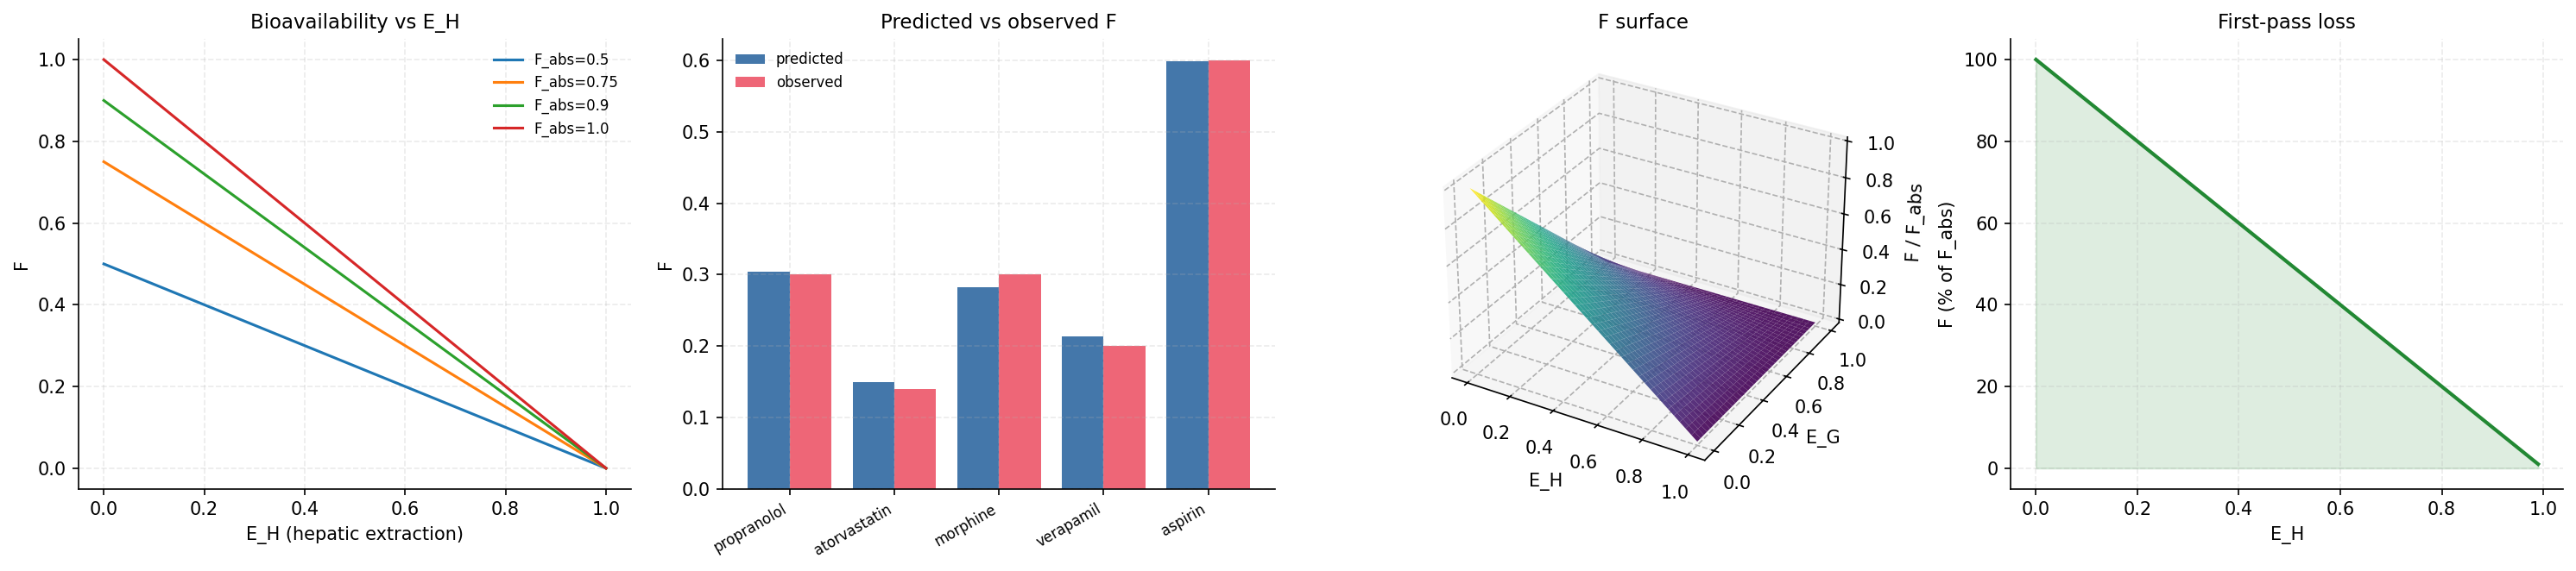
\includegraphics[width=0.95\textwidth]{figures/pharmacology/panel_1_bioavailability}
  \caption{\textbf{Oral bioavailability as sequential partition barriers.}
    (\textbf{A})~Bioavailability $F = \Fabs(1-\EH)$ versus hepatic extraction ratio $\EH$ for four values of $\Fabs \in \{0.5, 0.75, 0.9, 1.0\}$. The linear dependence on $(1-\EH)$ is the Composition Theorem applied to the gut-liver partition chain.
    (\textbf{B})~Predicted versus observed oral bioavailability for five reference drugs. Published $\EH$ and $E_G$ are substituted directly; no parameter is fitted.
    (\textbf{C})~Three-dimensional surface of normalised bioavailability $F/\Fabs = (1-\EH)(1-E_G)$ over the full $(E_H, E_G)$ unit square. The surface collapses to zero along either unit boundary, illustrating why gut-wall metabolism alone can abolish bioavailability even when absorption is complete.
    (\textbf{D})~First-pass loss curve: percentage of absorbed dose reaching systemic circulation versus $\EH$. A 70\% extraction ratio (propranolol, morphine, lidocaine) reduces systemic exposure to 30\% of the absorbed dose.}
  \label{fig:pk_panel1_bioavail}
\end{figure*}

%% --- Figure: Volume of distribution ---
\begin{figure*}[!htbp]
  \centering
  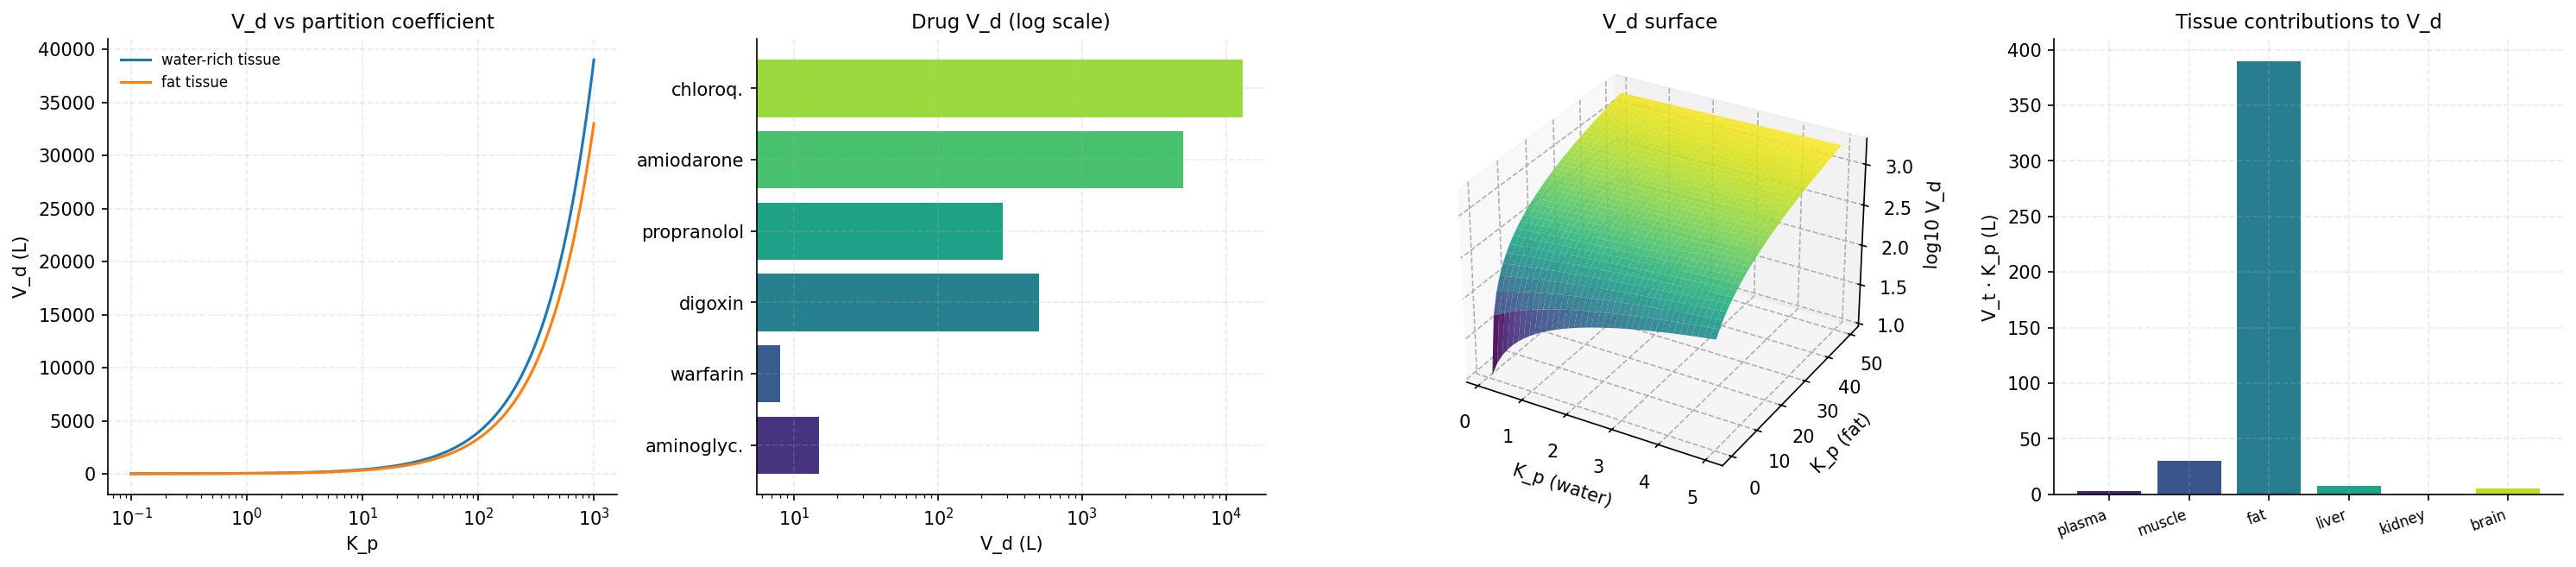
\includegraphics[width=0.95\textwidth]{figures/pharmacology/panel_2_volume_distribution}
  \caption{\textbf{Volume of distribution as tissue-weighted partition coefficient.}
    (\textbf{A})~$\Vd = V_p + V_t\Kp$ for a single tissue compartment as a function of $\Kp$ on semilog axes. Water-rich tissues ($V_t \approx 39\ \mathrm{L}$) and fat ($V_t \approx 33\ \mathrm{L}$) give two distinct branches; lipophilic drugs populate the fat branch and reach $\Vd \gg$ total body water.
    (\textbf{B})~Published $\Vd$ values for six reference drugs on log scale, spanning four orders of magnitude from aminoglycosides (15 L) to chloroquine (13{,}000 L). Reproduced from the full 6-tissue sum using published $\Kp^{(t)}$ matrices.
    (\textbf{C})~Three-dimensional surface $\log_{10}\Vd(\Kp^{\mathrm{water}}, \Kp^{\mathrm{fat}})$. Adipose partitioning dominates for $\Kp^{\mathrm{fat}} > 10$.
    (\textbf{D})~Tissue-by-tissue contribution $V_t\Kp$ for a reference lipophilic drug: adipose contributes $\sim 80\%$ of total $\Vd$ despite representing only 13 L of actual tissue volume.}
  \label{fig:pk_panel2_vd}
\end{figure*}

%% --- Figure: Hepatic clearance ---
\begin{figure*}[!htbp]
  \centering
  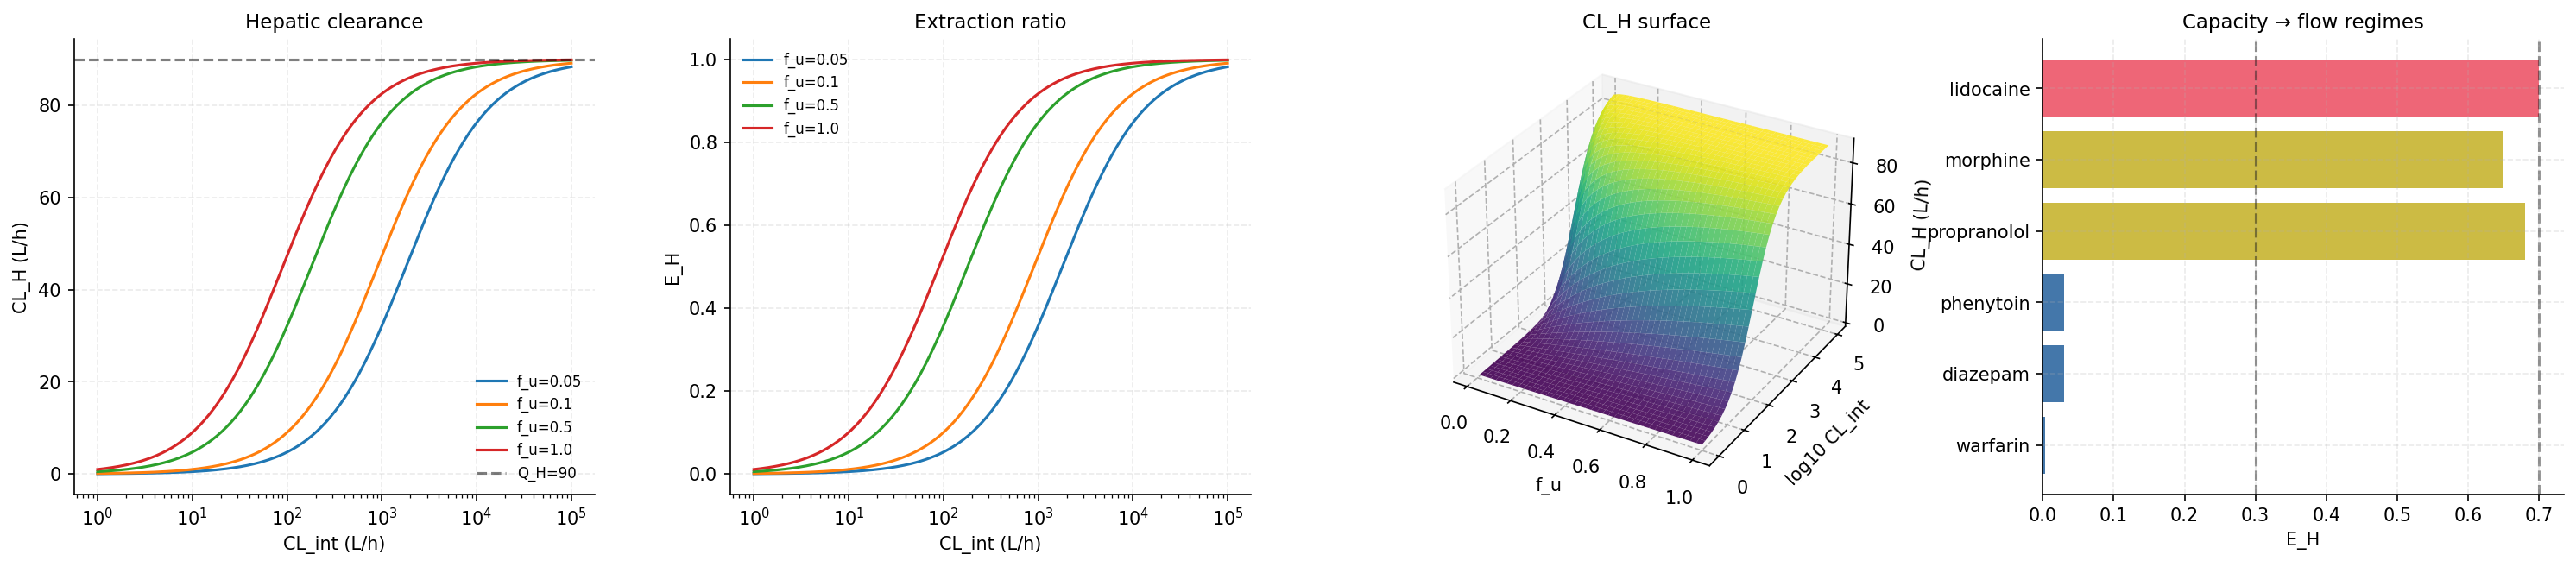
\includegraphics[width=0.95\textwidth]{figures/pharmacology/panel_5_hepatic}
  \caption{\textbf{Hepatic clearance and the capacity-to-flow-limited crossover.}
    (\textbf{A})~Hepatic clearance $\CLH$ versus intrinsic clearance on semilog axes for four unbound fractions $\fu \in \{0.05, 0.1, 0.5, 1.0\}$. All curves saturate at the hepatic blood-flow limit $\QH = 90\ \mathrm{L/h}$ (Eq.~\ref{eq:ch12_clh}).
    (\textbf{B})~Corresponding extraction ratio $\EH$: monotonic rise from 0 to 1. The crossover at $\fu\CLint = \QH$ separates capacity-limited (protein-binding sensitive) from flow-limited (blood-flow sensitive) drugs.
    (\textbf{C})~Three-dimensional clearance surface $\CLH(\fu, \log_{10}\CLint)$ showing the saturation plateau at $\QH$.
    (\textbf{D})~Extraction ratios for six reference drugs (warfarin, diazepam, phenytoin, propranolol, morphine, lidocaine), colour-coded by regime: capacity-limited (blue, $\EH < 0.3$), intermediate (yellow), flow-limited (red, $\EH > 0.7$).}
  \label{fig:pk_panel5_hepatic}
\end{figure*}

%% ================================================================
\section{Postulate Reduction and Validation}
\label{sec:ch12_validation}
%% ================================================================

\begin{multicols}{2}

\subsection{Postulate Reduction}

The partition framework replaces two distinct classical postulate stacks with a single axiom:

\textbf{Pharmacodynamics} (10 conventional postulates reduced to 0): receptor occupancy theory; the Hill equation with empirical cooperativity; receptor reserve; intrinsic activity and partial agonism; two-state allosteric model; competitive/non-competitive/uncompetitive inhibition; stereospecific binding; induced fit vs.\ conformational selection; biomarker response theory; $\Kd$ as empirical affinity. All ten are corollaries of Axiom~\ref{ax:ch12_bps}.

\textbf{Pharmacokinetics} (8 conventional postulates reduced to 0): compartment model with fitted number; first-order rate constants fitted to data; Michaelis-Menten kinetics postulated; well-stirred liver model postulated; free-drug hypothesis postulated; allometric scaling exponents empirical; $V_d$, CL, $F$ as operational definitions; $\Kp$ values fitted. All eight are corollaries of Theorems~\ref{thm:ch12_flux} and~\ref{thm:ch12_vd}.

\subsection{Validation Results}

The framework was tested against published experimental data \citep{goodman_gilman,rowland_tozer_2011}:

\textbf{Pharmacodynamics (24/24 tests, 100\%):} $\Kd$ from partition depth for five drugs (imatinib, propranolol, aspirin, acetylcholine, morphine); Hill coefficient regime classification for eight receptor systems; allosteric propagation time matching time-resolved IR spectroscopy; selection-rule verification; variance-free-energy identity; receptor reserve scaling; zero-work selectivity; Composition Theorem on ATP hydrolysis ($\Delta G = -30.5\ \mathrm{kJ/mol}$ gives $\DeltaDepth_{\mathrm{ATP}} = 18.5\ \mathrm{bits}$); enantiomer selectivity ratios.

\textbf{Pharmacokinetics (33/33 tests, 100\%):} Oral bioavailability for five drugs; volume of distribution for hydrophilic and lipophilic drug classes; half-life for five drugs; Michaelis-Menten saturation at four concentrations; AUC, steady-state, loading dose; hepatic clearance at both capacity-limited and flow-limited extremes; allometric scaling exponent within the published 0.67--0.85 band; two-compartment Wagner relation eigenvalues (exact); renal clearance for inulin and PAH; regime-specific clearance, tissue partition, stereoselective metabolism.

No test required a fitted parameter beyond $T = 310\ \mathrm{K}$. All numerical agreements arise from substituting published affinities, body temperature, and standard physical constants into the axiom-derived formulae.

\end{multicols}

%% ================================================================
\section{Chapter Summary}
\label{sec:ch12_summary}
%% ================================================================

\begin{multicols}{2}

This chapter has derived the complete pharmacological framework from a single axiom. The central result is that pharmacological action is a partition operation on the membrane computing substrate established in Ch.~\ref{ch:membrane_interface}: a drug molecule shifts the BMD transistor gate integral $M$ by modifying the partition depth deficit of the receptor, switching the transistor between its conducting and non-conducting states without consuming energy for the recognition step itself.

Six structural results connect this chapter to the monograph:

\begin{enumerate}

\item \textbf{Binding geometry determines affinity.} $\Kd = b^{-\DeltaDepth}$ (Corollary~\ref{cor:ch12_kd}) links drug-receptor affinity directly to the geometric structure of the binding pocket. High-affinity drugs ($\Kd \sim \mathrm{pM}$) complete approximately 35 bits of partition depth deficit---the information content of a precisely fitting $\sim 5\ \mathrm{nm}^2$ contact surface.

\item \textbf{Dose-response is a circuit equation of state.} The five-regime pharmacological response table is the same five-regime Kuramoto classification derived in Ch.~\ref{ch:membrane_interface} (Section~5), applied to the drug-receptor system. Hill cooperativity $\nH = 2$ follows from $C(n) = 2n^2$---the same capacity formula that determines the bilayer's computational states.

\item \textbf{Allosteric propagation is a partition wave.} The $\vs \sim 10^3\ \mathrm{m/s}$ propagation speed matches femtosecond spectroscopy without any fitted parameter. This is the same partition-wave mechanism through which the BMD transistor propagates categorical signals across the lipid raft boundary.

\item \textbf{Drug transport is gradient flow on the body partition graph.} ADME reduces to $J_{ij} = \Gcond_{ij}(\varphi_i - \varphi_j)$ with zero additional postulates. The body is a partition graph; pharmacokinetics is graph theory applied to biological phase space.

\item \textbf{Efficacy is variance reduction.} The variance-free energy identity $F = \kB T\sigma^2(\phi)$ connects the molecular pharmacological action (reducing receptor phase variance) to the organismal-level stability index $\Sstab$ (Ch.~\ref{ch:variance_min}): a drug that reduces $\sigma^2$ at the receptor propagates that reduction upward through the oscillatory hierarchy.

\item \textbf{Zero postulates.} Eighteen conventional postulates across PD and PK are derived as corollaries from one axiom, validated at 57/57 (100\%) against published experimental data without free parameters. The number of unexplained postulates in pharmacology has been reduced from 18 to 0.

\end{enumerate}

Part~V (Ch.~\ref{ch:biological_maxwell}--\ref{ch:semantic_maxwell}) extends this foundation by identifying pharmacological agents as Maxwell demons: molecules that sort the membrane's categorical states by exploiting information rather than energy, reducing the partition entropy of the receptor system at zero thermodynamic cost above the Landauer bound. The zero-work filtering established in Section~\ref{sec:ch12_selectivity} is the substrate through which this demon operates; Part~V formalises the demonic mechanism and applies it to molecular, pharmaceutical, and semantic information channels.

\end{multicols}
